\chapter{Collecting data in a computer}

In this assignment we will use some python libraries to receive the data transmitted by the sunset sensor in a computer instead of the Arduino.
You can use one of the university computers, a laptop or a RaspBerry.

Install the XBee python libraries.

\url{http://pypi.python.org/pypi/XBee/2.0.0}

This code offers an implementation of the XBee serial communication API.

We re-use the processing board of the previous assignment and this time we will connect the XBee that receives the data to the computer using the USB cable.
Remember that in the last assignment it was connected to the Arduino.

\begin{lstlisting} [caption = {Simple code that reads the message that arrive to the XBee.}, language = Python, label = {code:simple-receiver}, numbers = left, escapeinside={@}{@}]

import serial
from xbee import ZigBee

print 'Printing data from remote XBee'

serial_port = serial.Serial('/dev/ttyUSB0', 9600)
zigbee = ZigBee(serial_port)

while True:
    try:
        print zigbee.wait_read_frame()
    except KeyboardInterrupt:
        break

serial_port.close()
\end{lstlisting}

You can see the results of running the program in Fig. \ref{fig:sink_in_server_screenshot_first_test}.

\begin{figure}[htbp]
  \centering
  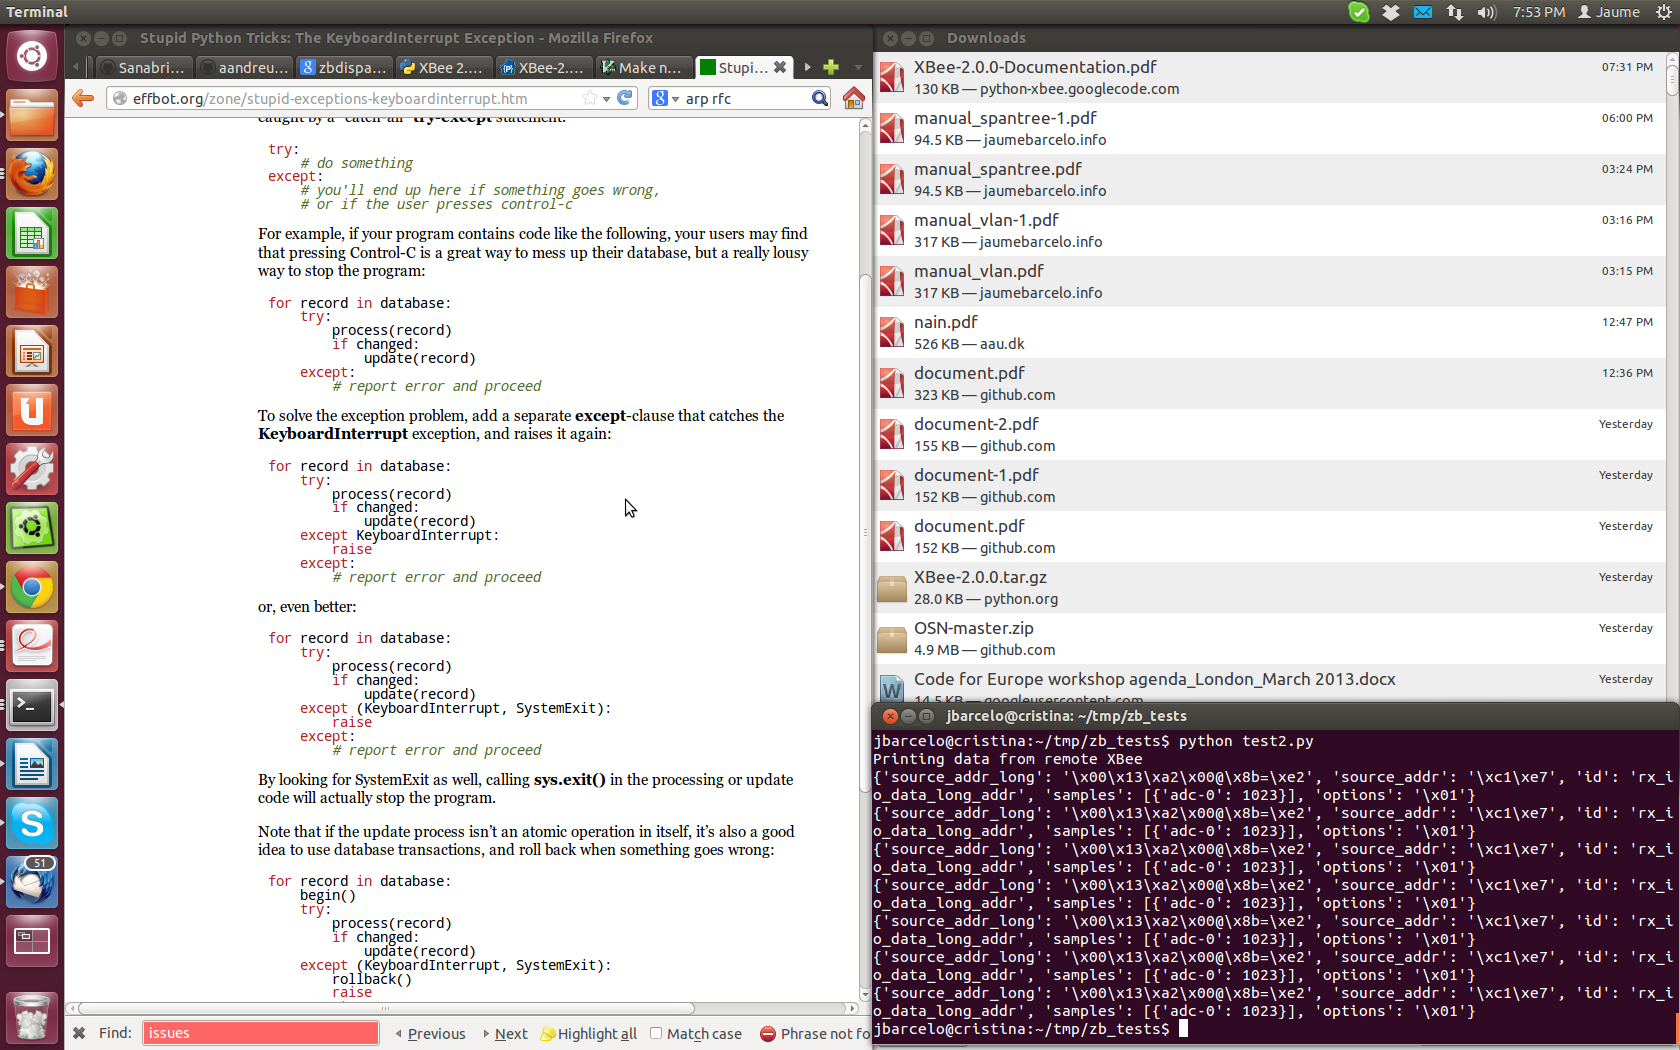
\includegraphics[width=0.7\linewidth]{figures/sink_in_server_screenshot_first_test.eps}
  \caption{A test run of a python program to read the messages that arrive to the XBee.}
  \label{fig:sink_in_server_screenshot_first_test}
\end{figure}


